\begin{frame}{De Bruijn Sequence (Positioning Sequence)}
    \begin{columns}
        \begin{column}{0.65\textwidth}
            \begin{enumerate}
                \vfill\item De Bruijn sequence:
                \begin{itemize}
                    \vfill\item A cyclic binary de Bruijn of order $k$ is a length $2^{k}$ sequence such that each length $k$ string appears exactly once.
                    \vfill\item Example: A de Bruijn sequence of order $4$.
                    
                    {\color{teal}Cyclic} : {\color{blue}0000100110101111}.

                    {\color{teal}Acyclic} : {\color{blue}0000100110101111000}.
                
                    \vfill\item De Bruijn sequence $\equiv$ longest simple path in de Bruijn graph (Eulerian cycle).
                    
                    
                \end{itemize}
                \visible<2->{
                \vfill\item De Bruijn graph of order $k$, $G_{k}$:
                \begin{itemize}
                    \vfill\item Each vertex is labeled by a sequence of length $k-1$.
                    \vfill\item A directed edge from $\bfx = \left[x_{0}x_{1}\ldots x_{k-2}\right]$ to $\bfy=\left[y_{0}y_{1}\ldots y_{k-2}\right]$ $\Leftrightarrow\ x_{1}x_{2}\ldots x_{k-2}=y_{0}y_{1}\ldots y_{k-3}$. 
                \end{itemize}
                }
            \end{enumerate}
        \end{column}
        
        \visible<3->{
        \begin{column}{0.35\textwidth}
            \begin{figure}
                \centering
                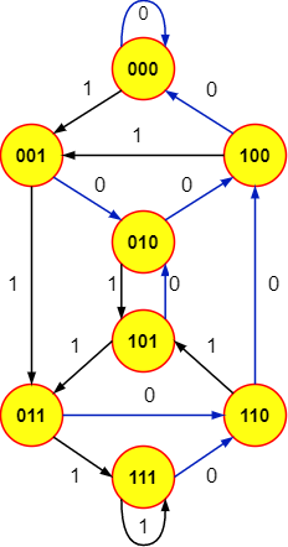
\includegraphics[width=0.75\textwidth]{Images/deBruijnOrder4.png}
                \caption{de Bruijn graph of order $4$.}
                \label{fig:dB4}
            \end{figure}
        \end{column}
        }
    \end{columns}
\end{frame}

\begin{frame}{Run Length Limited de Bruijn (RdB) sequences}
    \begin{definition}
        A $(k,s)$-RdB sequence: a de Bruijn sequence of order $k$ containing at most $s$ consecutive bit $0$'s.
    \end{definition}
    \begin{overprint}
        \onslide<1> 
            Trivial cases:
            \begin{itemize}
                \item $s\geq k$: original de Bruijn sequence.
                \item $s=k-1$: remove $0^{k-1}$ in the de Bruijn graph.
            \end{itemize}
            $\Rightarrow$ Interested in:
            \begin{itemize}
                \item $s<k-1$: eliminate vertices with more than $s$ consecutive bit $0$'s.
            \end{itemize}
        \onslide<2->
            \begin{columns}
            \visible<2->{
                \begin{column}{0.33\textwidth}
                    \begin{figure}[htbp]
                        \centering
                        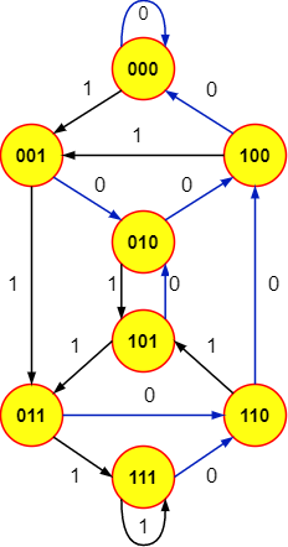
\includegraphics[scale=0.27]{Images/deBruijnOrder4.png}
                        \caption{de Bruijn graph of order $4$.}
                        % \label{fig:my_label}
                    \end{figure}
                \end{column}
            }
            \visible<3->{
                \begin{column}{0.34\textwidth}
                    \begin{figure}[htbp]
                        \centering
                        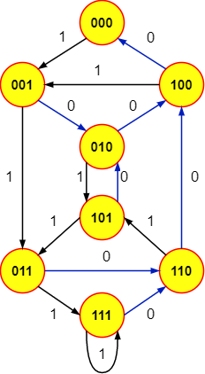
\includegraphics[scale=0.35]{Images/RdB/RdB_4_3.png}
                        \caption{$(4,3)$-RdB graph.}
                        \label{fig:RdB_4_3}
                    \end{figure}
                \end{column}
            }
            \visible<4->{
                \begin{column}{0.33\textwidth}
                    \begin{figure}[htbp]
                        \centering
                        % 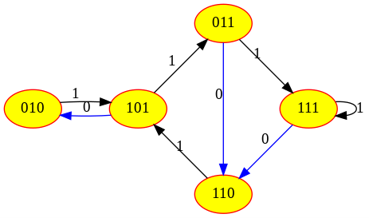
\includegraphics[scale=0.4]{Images/RdB/RdB_4_1.png}
                        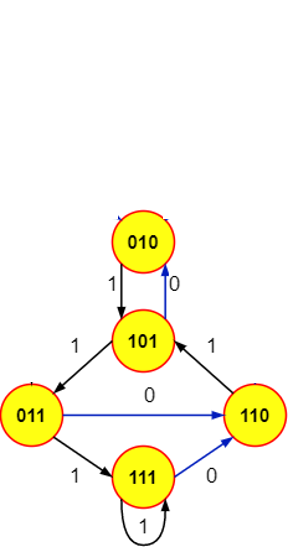
\includegraphics[scale=0.26]{Images/RdB/4_1_RdB.png}
                        \caption{$(4,1)$-RdB graph.}
                        \label{fig:RdB_4_1}
                    \end{figure}
                \end{column}
            }
        \end{columns}
    \end{overprint}
    
    
\end{frame}

\begin{frame}{Maximal length of $(k,s)$-RdB sequence}
    Given $k,s$. Notations:
    \begin{itemize}
        \item $\ell(k,s)$: maximal length of simple path $(k,s)$-RdB graph.
        \item $N(k,s)$: maximal length of $(k,s)$-RdB sequences $(=\ell(k,s)+k-1)$.
    \end{itemize}
    \begin{theorem}
        Given $k,s$. Then:
        \begin{align}
            \ell(k,s) = \card{W(k,s)} - \left(\sum_{i=0}^{C}(s-i)\card{W(k-s-i-3,s)}-s\right)
        \end{align}
    \end{theorem}
    where :
    \begin{itemize}
        \item $C=\min(s-1,k-s-2)$.
        \item $W(n,s)$: set of length $n$ sequences containing at most $s$ consecutive bit $0$'s. 
    \end{itemize}
\end{frame}

\begin{frame}{Maximal length of $(k,s)$-RdB sequence}
    \begin{lemma}
        \centering
        $\ell(k,s)\leq\card{W(k,s)} - \left(\sum_{i=0}^{C}(s-i)\card{W(k-s-i-3,s)}-s\right) $
    \end{lemma}
    Observe:
    \begin{itemize}
        \item Vertices: balanced, right-unbalanced, left-unbalanced.
        \item Number of left(right)-unbalanced vertices of form $0^{s}1\ldots10^{i}$ is $\card{W(k-i-s-3,s)}$ with $i\leq C=\min(s-1,k-s-2)$.
    \end{itemize}
    \begin{figure}
        \centering
        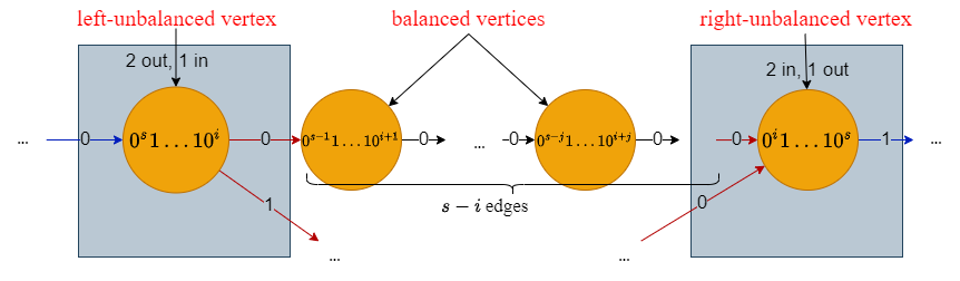
\includegraphics[width=0.9\textwidth,height=.3\textheight]{Images/Rate/sketchproof.png}
        \caption{Vertices in RdB graphs.}
        \label{fig:sketchproof}
    \end{figure}
\end{frame}